% Compiler ce document 

% package de base
\documentclass[10pt,a4paper]{article}
\usepackage[utf8]{inputenc}
\usepackage{listings}

% langues
\usepackage[usenames,dvipsnames]{xcolor}
\usepackage[francais]{babel}
\usepackage[T1]{fontenc}
\usepackage{amsmath}
\usepackage{amsfonts}
\usepackage{amssymb}
\usepackage{graphicx}
\usepackage{tabularx}
\usepackage{colortbl}
\usepackage[hidelinks]{hyperref} % liens
\usepackage{fancyhdr} % En tetes / bas de page
\usepackage{helvet} % police helvetica
\usepackage[hidelinks]{hyperref}
\usepackage{xcolor} % Style pour affichage du C
\usepackage{courier} % police pour les listings

\usepackage{listingsutf8}

% Page de Garde -- Necessite d'installer le package titling, si probleme
% commenter la ligne suivante ainsi que les infos necessaires a la page
% de garde
\usepackage{pageGarde/HEIG_STY}

% commande pour faire des sections sans nombre 
% tout en la rajoutant dans la table des matières
\newcommand\sectionWithoutNumber[1]{\section*{#1} \addcontentsline{toc}{section}{\protect\numberline{}#1}}
\newcommand\subsectionWithoutNumber[1]{\subsection*{#1} \addcontentsline{toc}{subsection}{\protect\numberline{}#1}}
\newcommand\subsubsectionWithoutNumber[1]{\subsection*{#1} \addcontentsline{toc}{subsubsection}{\protect\numberline{}#1}}
% définition de nouvelles couleurs
\definecolor{lightblue}{rgb}{0.8,0.8,0.9}
\definecolor{grossblue}{rgb}{0,0,0.7}
%marge des pages
\setlength{\textwidth}{16cm}
\setlength{\textheight}{24cm}
\setlength{\oddsidemargin}{0cm}
\setlength{\voffset}{-1.5cm}
\setlength{\headheight}{15pt}

% set la police en arial
%% Sans-serif Arial-like fonts
\renewcommand{\rmdefault}{phv} 
\renewcommand{\sfdefault}{phv} 
\usepackage{tabularx}
\usepackage{graphicx}
\usepackage{eurosym}
\usepackage{xspace}
\newcommand{\projectname}[0]{LTANR\xspace} 

% configuration pour des listings
\lstset{ 
  showspaces=false,      
  showstringspaces=false, 
  showtabs=false,               
  tabsize=3,                     
  numbers=left
}

%enlève indentation en début de paragraphe
\setlength\parindent{0pt}

%style de l'en-tête de page
\pagestyle{fancy}

% style pour code en c
\lstdefinestyle{customc}{
  belowcaptionskip=1\baselineskip,
  breaklines=true,
  frame=L,
  xleftmargin=\parindent,
  language=C,
  showstringspaces=false,
  basicstyle=\scriptsize\ttfamily,
  keywordstyle=\bfseries\color{green!40!black},
  commentstyle=\itshape\color{purple!40!black},
  identifierstyle=\color{blue},
  stringstyle=\color{orange},
}

\lstdefinelanguage{VHDL}{
      morekeywords=[1]{
        library,use,all,entity,is,port,in,out,end,architecture,of,
        begin,and,or,Not,downto,ALL
      },
      morekeywords=[2]{
        STD_LOGIC_VECTOR,STD_LOGIC,IEEE,STD_LOGIC_1164,
        NUMERIC_STD,STD_LOGIC_ARITH,STD_LOGIC_UNSIGNED,std_logic_vector,
        std_logic
      },
      morecomment=[l]--
    }
    \usepackage[usenames,dvipsnames]{xcolor}
    \colorlet{keyword}{blue!100!black!80}
    \colorlet{STD}{Lavender}
    \colorlet{comment}{green!80!black!90}
    \lstdefinestyle{vhdl}{
      language     = VHDL,
      basicstyle   = \footnotesize \ttfamily,
      keywordstyle = [1]\color{keyword}\bfseries,
      keywordstyle = [2]\color{STD}\bfseries,
      commentstyle = \color{comment}
      breaklines=true,                % sets automatic line breaking
      tabsize=3                                % sets default tabsize to 2 spaces
    }

\lstset{escapechar=@,style=customc}
\lstset{inputencoding=utf8/latin1} %affiche les accents dans le listing

% Mise en forme de la page de titre
\author{João Miguel Domingues Pedrosa \\
Loïc Haas\\
Rick Wertenbroek}
\title{PCAP et Drum Challenge \\ Laboratoire 1}
\dest{Laboratoire 1}

% Informations necessaires a la page de garde
% Commenter si probleme de compilation
\acro{MCS}
\matter{Modern Concurent System}
\date{\today}

%en-tête
\lhead{João, Loïc \& Rick}
\chead{Laboratoire 1}
\rhead{\theAcro}

%pied-de-page
\lfoot{HEIG-VD}
\cfoot{\today}
\rfoot{\thepage}

\begin{document}
\maketitle
\newpage
\tableofcontents
\newpage

%Ici commence réelement l'écriture du rapport

\section{Drum challenge}

\subsection{Résume du problème}

L'objectif de ce challenge est de pouvoir recomposer l'affichage d'un des valeurs d'un fichier contenant les informations sous forme binaire. Il y a que pour seul aide les informations sur comment ça doit s'afficher et donc quelle sont les champs qui doivent apparaître.

\subsection{Décomposition du fichier binaire}

Les valeurs à décoder sont contenu dans un fichier possédant l'extension \texttt{.splice}. Il en a été fournit 5 avec leur équivalent lors de l'affichage du format.\\

Pour m'aider dans la recherche de la décomposition des informations, on a utilisé le logiciel \texttt{hexinator} permettant l'affiche du contenu d'un fichier en valeur hexadécimal.

\begin{figure}[htc]
	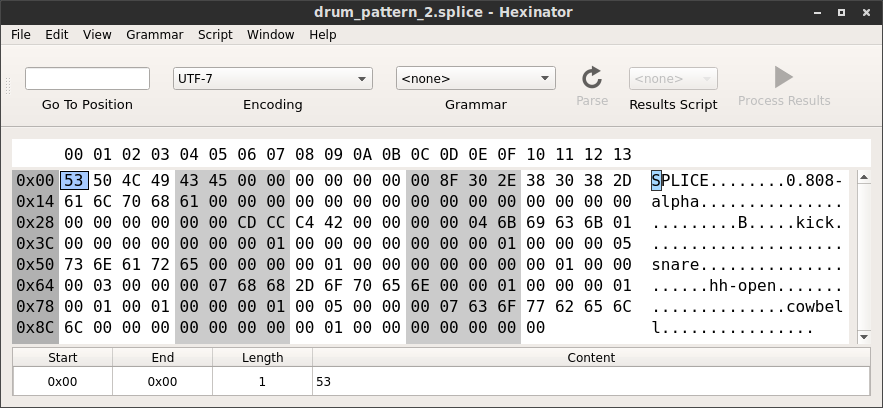
\includegraphics[scale=0.51]{images/hexa.png}
	\caption{Exemple de se que nous sort Hexinator}
\end{figure}

Avec la comparaison des différents fichiers fournit avec leur format d'affiche nous avons retiré les informations suivantes:
\begin{itemize}
    \item Header
    \begin{itemize}
		\item 6 octet: magic word (indique le type fichier)
		\item 8 octet: longueur en octet des informations restantes
		\item 32 octet: Nom de la version hardware (big-endian)
		\item 4 octet: tempo en float (little-endian)  
    \end{itemize}
    
    \item Tracks	
    \begin{itemize}
    	\item 1 octet: identifiant numérique
    	\item 4 octet: taille du nom de l'instrument (big-endian)
    	\item n octet: nom de l'instrument 
    	\item 4 * 4 octet: la mesure décomposer en 4 quarter de 4 battement
    \end{itemize}
\end{itemize}

À noter que les information arrivent dans ce même ordre. La taille du header est constant pour chaque fichier. Par contre les tracks changent, déjà parce qu'il peut y en avoir plusieurs dans un fichier et le nom de l'instrument varie aussi.

\newpage

\subsection{Parsing des informations}

\subsubsection{Header}
Pour pouvoir parser le header, nous avons fait la fonction suivant:

\lstinputlisting[firstline=54, lastline=60,language=erlang]{sources/drum_sample.erl}

Nous commençons par regarder si le magic word est juste sinon on revoit un tuple contenant le type d'erreur et le binaire en brute. On récupére un payload de la taille définit par la valeur lu précédement. Il a été fait ainsi car il n'est pas impossible d'avoir des octet en trop, cela n'est pas considérer comme une erreur. Ils doivent être ignorer d'où le dernier match. Un exemple et trouvable dans le 5ème fichier pattern:

\begin{figure}[htc]
	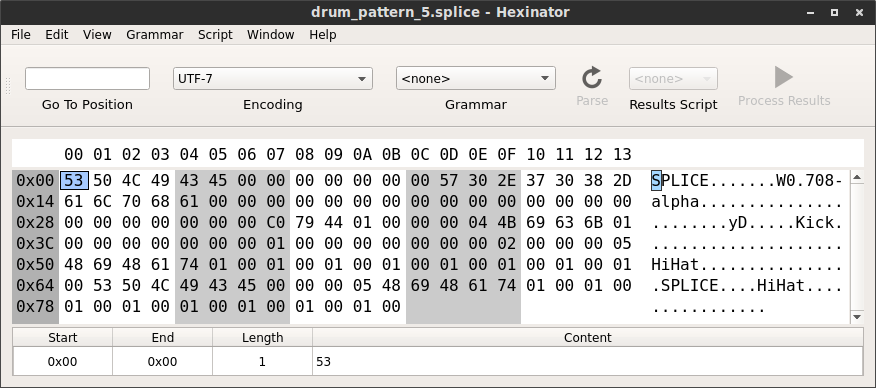
\includegraphics[scale=0.51]{images/hexa_fail.png}
	\caption{Ici, le payload fait 87 octet, en regardant bien, on voie que l'on en a plus}
\end{figure}

Si la matching est juste, on récupère la version du hardware, le tempo et les tracks via un pattern matching avec le payload puis on retourne tout ça avec un tuple.

\subsection{Tracks}
Pour parser les tracks, nous avons décomposé en 2 fonctions, une qui se charge de faire la base (récupérer l'identifiant et le nom) et une autre pour la décomposition de la mesure.\\

Premièrement, la fonction pour le track complet:

\lstinputlisting[firstline=64, lastline=71,language=erlang]{sources/drum_sample.erl}

\newpage

Cette partie se charge récupérer sous forme d'une liste composer de tuple id, nom de l'instrument et les mesures. Elle ne s'arrête que quand le binaire passé en argument est vide.

Ensuite, pour récupérer les mesures, on utilise la fonction suivante:

\lstinputlisting[firstline=75, lastline=86,language=erlang]{sources/drum_sample.erl}

Ici, on va lire récursive le binaire passer jusqu'à ce qu'il soit vide. On récupère un quarter à la fois au quel on vérifie que chaque valeur soit 1 ou 0 sinon ça veut dire que le fichier est mal formé et qu'il y a une erreur. On revoit une liste contenant les quarter qui sont eux aussi des listes de 0 et 1.

\subsection{Rendu des information}

Pour le le format de l'affiche, on a fait la fonction suivante:

\lstinputlisting[firstline=90, lastline=92,language=erlang]{sources/drum_sample.erl}

On lui passe la version, le tempo et les tracks que l'on fait passer dans un format afin d'avoir un affichage correcte. L'affichage du tempo se fait ainsi, s'il y a des valeurs après la virgule on les affiches sinon on affiche juste la valeur entière. Erlang n'arrivant pas à le faire de base, on passe par une fonction intermédiaire qui se charge de détecter et renvoyer le bon format:

\lstinputlisting[firstline=142, lastline=146,language=erlang]{sources/drum_sample.erl}

Ensuite, pour les tracks, nous devons tout d'abord trouver le nombre d'espace à mettre entre le nom de l'instrument et les mesures (padding). Nous avons trouvé que entre 2 fichier (exemple: le pattern 1 et 4), l'espace minimum étaient différent. L'explication que nous avons trouvé à cela était que si la première lettre de l'instrument est en majuscule alors l'écart est plus grand. Ce qui donne la fonction suivante:

\lstinputlisting[firstline=150, lastline=158,language=erlang]{sources/drum_sample.erl}

On vérifie pour chaque instrument s'il y en a un qui commence par une majuscule au quel cas on renvoit ne nombre d'espace à ajouter.\\

La fonction pour le format des tracks est le suivant:

\lstinputlisting[firstline=96, lastline=125,language=erlang]{sources/drum_sample.erl}

Le premier en-tête se charge de récupérer le nombre de caractère requit pour avoir les mesures en colonnes sur chaque ligne. On récupère la longueur du nom de l'instrument le plus grand et l'ID le plus grand. On additionne ces valeurs au padding. Avec ceci, on pourra calculer le nombre d'espace à ajouter entre le nom et les mesures de l'instrument.\\

Ensuite, pour le format, on met l'ID entre parenthèse suivie du nom, après il y a le nombre d'espace à rajouter (on crée un tableau fait que d'espace) et on fini avec les mesure qui sont traité dans une fonction à part étant la suivante:

\lstinputlisting[firstline=129, lastline=138,language=erlang]{sources/drum_sample.erl}

On crée juste un tableau remplaçant les 0 par des - et les 1 par des x. On accumule une liste des ces tableau jusqu'à ce que l'on est plus  à traiter.\\

\subsection{Lecture de fichier}

Pour le décodage du fichier, on utilise la fonction suivante:

\lstinputlisting[firstline=34, lastline=42,language=erlang]{sources/drum_sample.erl}

On se charge juste de parser les valeurs afin de récupérer les informations nécessaire au rendu final. On peut aussi directement obtenir l'affichage à partir du fichier. Il se charge juste d'utilisé la fonction précédente et utilise la fonction \texttt{render} avec les informations récupéré.

\lstinputlisting[firstline=26, lastline=32,language=erlang]{sources/drum_sample.erl}

\end{document}
